%!TEX root = ../NCVC4.tex

\mysection{基本生成}

\subsection{CADでの作図}
 ワイヤ放電加工機用のNCデータ生成における、基本的な作図方法を解説します。
既知部分は省略されていますので『NCVC解説書』か、著書『いまからはじめるNC工作』も併せて参照してください。

%\begin{figure}[H]
%\centering
%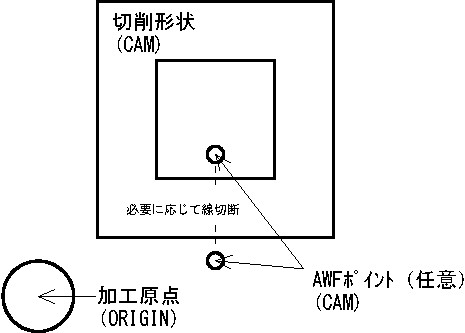
\includegraphics{No1/fig/sample1-crop.pdf}
%\caption{サンプル図形}
%\label{fig:sample1.pdf}
%\end{figure}

 基本はマシニング加工での作図と変わりありませんが、新たにAWF(自動結線機構)のポイントが指示できるようになっています。
無くてもOKですし、あればそこへ移動してワイヤ結線の指示ブロックが挿入されます。
円データで指示してください。
どの円データが対象になるかは加工条件で指示します。

 生成方法もマシニング加工と変わりありませんが、例えば仕上げしやすいように平面での切り始めにしたい場合は、該当部分で線を切断(分割)して端点を作り出してください。
図\ref{fig:sample1.pdf} の例で言うと、点線での線切断が無いと従来通り一番近い端点、つまり左下の角(カド)からの切削スタートになります。

 切削データはAWFポイント含め、1つのレイヤに作図してください。
2つのレイヤに作図すると上下異形状切削と認識されます。図\ref{fig:sample1.pdf} の点線は補助線です。念のため。

\subsection{形状認識処理}
 単一レイヤでの基本生成の場合、この処理は無くても生成できますが、次の上下異形状切削では必須なので、基本生成においても操作する癖をつけておいてください。
\menu{編集>加工指示>形状認識処理}(\,\keys{Ctrl+E}\,)を選択すると図\ref{fig:keijyo.png} のようにウィンドウの右側に連続線の図形集合(プリミティブ)が追加されます。

 『自動輪郭処理(手抜き)解説書』にもある通り、マシニング加工用には輪郭オフセット等を設定するための前処理ですが、ワイヤ放電加工機用でも使います。
主に方向指示と開始位置の指示を使います。というか、輪郭加工やポケット加工の指示はワイヤ放電加工機用には使えません。

%\begin{figure}[H]
%\centering
%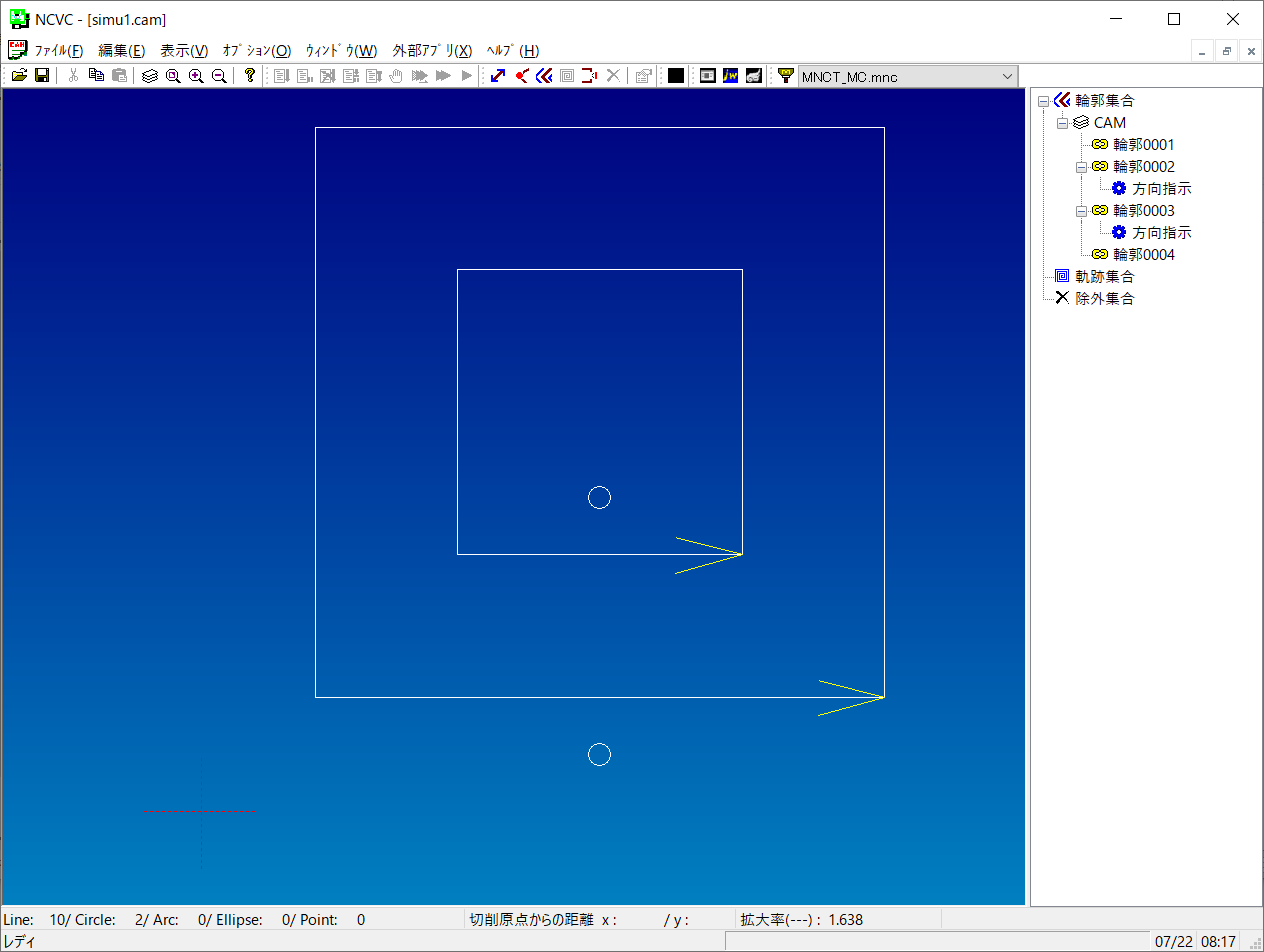
\includegraphics{No1/fig/keijyo.png}
%\caption{形状認識処理}
%\label{fig:keijyo.png}
%\end{figure}

 方向指示などを適当に加えてください。
\menu{ファイル>加工情報の保存}(\,\keys{Ctrl+S}\,)でこの状態を保存できます。

\subsection{加工条件の設定}
 切削レイヤ情報が2つ以下の場合に限り、
\menu{ファイル>NCデータの生成>ワイヤ放電加工機データの生成}(\,\keys{Shift+Ctrl+Alt+F7}\,)が有効になります。

\begin{minipage}[t]{0.4\textwidth}
 ワイヤ放電加工機用の条件ファイルは拡張子が(ncw)です。
基本タブがワイヤ加工機用に変更されている他、AWFタブが新設されています。
AWFタブにはワイヤの結線や切断の任意コードが設定でき、対象となる円の半径を範囲で指定します。
生成と表記のタブはほぼ従来通りです。

 テーパ角度の設定は、切削レイヤが1つの場合に限ります。
\end{minipage}
\begin{minipage}[t]{0.6\textwidth}
%\vspace*{-2zh}
%\begin{figure}[H]
%\centering
%\includegraphics[scale=0.7]{No2/fig/ncw.png}
%\caption{加工条件の設定}
%\label{fig:ncw.png}
%\end{figure}
\end{minipage}

\vspace*{1zh}
 ここで、カスタムヘッダー・フッターについて解説します。
旋盤データの生成と同様に、ワイヤ放電加工機用にも置換キーワードが追加されていますので、ご確認ください。

\begin{minipage}[t]{0.6\textwidth}
\begin{lstlisting}[caption=Header.txt,numbers=none,label=lst:header.txt]
%
{ProgNo}
({MakeDate} {MakeTime})
({MakeUser} MADE {MakeNCD} FROM {MakeDXF} ⇒
                           AND {MakeCondition})
(WireView={WorkDepth})
{TaperMode}
{G90orG91}{G92_Initial}I{WorkDepth}
\end{lstlisting}
\end{minipage}
\begin{minipage}[t]{0.4\textwidth}
\begin{lstlisting}[caption=Footer.txt,numbers=none,label=lst:footer.txt]
G50T0{G0XY_Initial}U0V0
M30
%
\end{lstlisting}
\end{minipage}

\begin{table}[H]
\centering
\caption{置換キーワード}
\label{tab:keyword}
\begin{tabular}{|p{3cm}|p{10cm}|}
\hline
ProgNo & 加工条件の[生成]タブにあるプログラム番号に置換 \\ \hline
WorkDepth & 基本タブの[ワーク厚み]に置換 \\
TaperMode & 基本タブの[テーパモード]に置換 \\ \hline
\end{tabular}
\end{table}

\subsection{Gコードの生成}
 あとはOKボタンで完了です。
カスタムヘッダーにワイヤ放電加工機用の表示切り替えキーワードを埋め込んでいるので、生成後即ソリッド(ワイヤモードの場合は面のみ)表示が可能です。

%\begin{figure}[H]
%\centering
%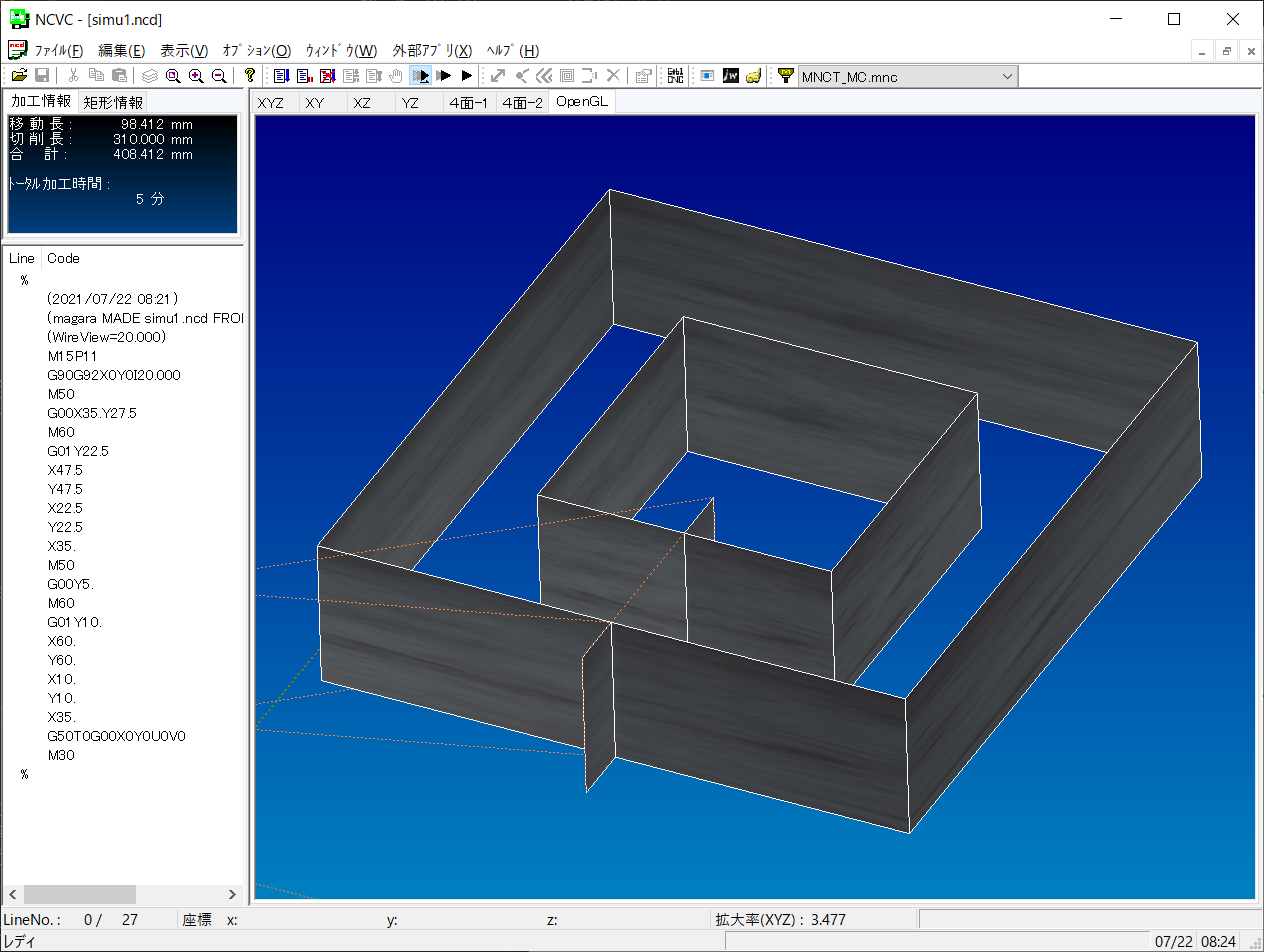
\includegraphics[scale=0.5]{No1/fig/simu1.png}
%\caption{Gコードシミュレーション画面}
%\label{fig:simu1.png}
%\end{figure}

 当たり前ですが、中抜きの場合は先に内側が処理され、最後に外側が処理されます。
こういう関連する図形同士の場合は、輪郭集合に属している場合のみ効力を発揮します。
交点や閉ループでない軌跡集合では、近さが優先されます。

\vspace*{3zh}
\begin{itembox}[l]{ここまでの【まとめ】}
(1) CADでの作図
\begin{itemize}
\item 基本は従来通り。必要に応じて線切断等の処理を行う
\item AWFポイントは円データで指示する(省略可)
\item テーパ角度指定は切削レイヤが1つの場合のみ
\end{itemize}
(2) 形状認識処理
\begin{itemize}
\item できるだけ輪郭集合に属するよう、交点のない閉ループで作図
\item 方向指示や加工開始位置の指示はマシニング加工でも使えます
\end{itemize}
(3) 加工条件とシミュレーション
\begin{itemize}
\item ワイヤ放電加工機用の加工条件(ncw)で設定する
\item カスタムヘッダーが適切に設定されていると、生成後即ソリッド表示が可能
\end{itemize}
\end{itembox}
